\documentclass[12pt]{article}

\usepackage{sbc-template}
\usepackage{graphicx,url}
\usepackage[utf8]{inputenc}
\usepackage[brazil]{babel}
\title{Algoritmos de Busca no Pac-Man \\
Introdução à Inteligência Artificial}

\author{Vinicius Julião Ramos - 2018054630}


\address{Departamento de Ciência da Computação \\Universidade Federal de Minas Gerais
(UFMG)
\email{viniciusjuliao@dcc.ufmg.br}
}

\begin{document} 
\maketitle


\section{Introdução}

O presente trabalho constituído pelo desenvolvimento e análise da aplicação
de algoritmos de busca sobre o jogo Pac-Man.
Essa atividade tem como fim a introdução de algoritmos utilizados por
inteligências artificiais em problemas reais, como um \textit{video game}.
Além disso, tal aplicação só é possível graças à modelagem do problema, em que
o estado do jogo se dá pelas posições disponíveis no tabuleiro (mapa),
sendo que os estados considerados como estados objetivos, são aqueles que
contêm a "comida" do personagem.

No jogo, o personagem pode mudar de posição apenas para aquelas posições
ajacentes à posição atual.
Tal adjacência se dá pelas posições acima, abaixo, à esquerda e à direita.
Logo, cada estado tem no máximo quatro outros estados descendentes.
É importante destacar que o mapa não é infinito, ou seja, há barreiras que
impedem o personagem de realizar um movimento, logo é possível que
determinados estados tenham menos de quatro estados descendentes.
Dessa forma, é possível caminhar de forma sistêmica em todo este grafo a fim
de alcançar os estados objetivos, e vencer o jogo.

Apesar da simplicidade do solucionador de um jogo 2D, a busca em grafos é
utilizada em diversas aplicações muito complexas, mas, em linhas gerais, tem
implementação relativamente simples.
Outro fator de importância dos algoritmos de busca, é à adaptabilidade para
diferentes tipos de problemas, enquanto há aqueles que são aplicáveis a
qualquer problema, há outros que demandam maior conversão de especificidade.
Um bom exemplo são os algoritmos \textbf{BFS} e \textbf{A*}, no qual o primeiro
pode ser aplicado de maneira genérica em muitos tipos de busca em grafos.
Já o segundo algoritmo, demanda a criação de uma função heurística, o que
desperta a necessidade de entender do comportamento das instancias
que o algoritmo resolve, a fim de que essa função heurística seja capaz
de optimizar a busca.

\section{Soluções}
De maneira geral, como trata-se de buscas em grafos, este tralho desenvolveu
três estruturas diferentes de solucionadores que serão apresentadas em
ordem a seguir.
As duas primeiras, são buscas que não desconsideram custos na troca de estados,
entretanto, cada uma delas tem a própria maneira de expansão de nós.
Já a ultima estrutura, que fora utilizada para três algoritmos diferentes,
atribui pesos às mudanças de estado de maneira a optimizar -- minimizar --
a quantidade de nós expandidos.

\subsection{Busca em Profundidade}
Este é um algoritmo recursivo, que não considera custos de transições de
estado, assim como mostram \cite{cormem} e \cite{livro-texto}.
A composição algorítmica desta solução, faz com que a partir de um determinado
nó, de maneira recursiva, visite-se imediatamente os nós vizinhos (que ainda
não foram visitados).
Ao imaginar uma árvore de decisão, em que os nós da árvore são os estados do
problema e as arestas são as decisões de transições tomadas pelo algoritmo,
a busca em profundidade parte da raiz (estado inicial) visitando primeiramente
todo um ramo da árvore, antes de visitar quaisquer outros nós.
Ao se deparar com um nó folha, atinge-se a condição de parada da recursão,
e então, parte-se para a visitação do \textit{sub-ramo} que descende do pai
daquele nó folha.
Contanto, a condição de parada que o algoritmo busca é o nó que identifica
o estado objetivo do problema.
Ao alcançar este ponto, o algoritmo é finalizado.

Apesar da característica recursiva do problema, o código desta solução não
foi desenvolvido com chamadas recursivas.
É possível utilizar uma estrutura de \textbf{pilha} para a visitação em
profundidade, então optou-se por esta solução, uma vez que o empilhamento
de chamadas recursivas adiciona uma sobrecarga muito grande na solução.
Em instancias muito grandes, a árvore de decisões pode conter diversos níveis
e para cada nível, adicionaria-se uma chamada de função, sobrecarregando
a solução com a criação de novas variáveis.
A solução chamada iterativa, necessita apenas de armazenar os dados de cada
nó (estado) que será visitado a posteriori.

Por fim, utilizou-se também uma segunda pilha para armazenar a sequencia de
tomadas de decisão realizadas pela busca em profundidade.
Cada vez que a solução se aprofunda um nível da árvore de decisões, armazena-ze
aquele aprofundamento.
Da mesma maneira, ao voltar um nível (emergir), a ultima decisão armazenada
na pilha é removida.
Enfim, ao encontrar o nó objetivo e parar a busca em profundidade, a pilha
de decisões armazenou o passo a passo de como sair do nó raiz e chegar até
o objetivo.

\subsection{Busca em Largura}
Em contraste com a busca em profundidade, nesta solução, a visitação
da árvore de decisão é realizada de maneira "ramo a ramo".
Na verdade, deseja-se visitar a árvore de decisões nível a nível.
Ou seja, para que um nível $i+1$ seja visitado, é necessário que todos
os nós do nível $i$ já tenham sido visitados anteriormente.
A implementação dessa característica de visitação, requer o uso de uma
estrutura de \textbf{fila}, em que, ao visitar um nó $n$, adiciona-se
ao final da fila todos os nós filhos de $n$.
Em questões práticas, ao expandir o estado $s$, todos os estados vizinhos
de $s$ são adicionados ao fim da fila.

Através dessa expansão em largura, pode-se chegar até o nó objetivo.
Contudo, é preciso lembrar de uma restrição que fora adicionada a todas
as soluções: Um estado não deve se expandido mais de uma vez, ou seja,
na árvore de decisões não visitamos o mesmo nó mais de uma vez.
Diferentemente da visitação em profundidade, a qual a própria pilha de
visitação armazena as transições que a solução deve apresentar,
na busca em largura é necessário utilizar uma estrutura mais complexa.
Optou-se pela implementação de um dicionário, no qual, após expandir
determinado nó, armazenamos aquele nó no dicionário, mapeando o
nó pai.
Dessa maneira, para obter a sequencia de decisões (a solução), desde que o
nó objetivo fosse encontrado, bastou caminhar no dicionário em
direção ao nó raiz da árvore de decisões.

\subsection{Busca em Transições Ponderadas}
As outras três soluções apresentadas por este trabalho consideram o peso
da transições ou pesos dos estados ao realizar a visitação dos nós da árvore
de decisão.
Estes algoritmos são \textbf{A*}, \textbf{Greedy}, e
\textbf{Uniform Cost Search}, os quais possuem a mesma estrutura básica, sendo
que a única mudança é a função que avalia a qualidade da transição, assim como
mostrado em \cite{livro texto}.

Neste ponto, houve a necessidade de utilizar a estrutura
\textbf{fila de prioridades}, na qual a função \textit{custo de transição}
define a ordem de expansão dos estados.
Ou seja, cada vez que um estado é expandido, os estados vizinhos são
adicionados à fila de prioridades, sendo que o \textit{custo de transição}
é definido pelo respectivo algoritmo, dentre aqueles três que realizam
tal ponderação.
Exatamente como na busca em largura, a estrutura de dicionário também fora
utilizada para armazenar a sequência de visitação.
Assim que um nó é visitado, ele é adicionado ao dicionário mapeando o nó
predecessor.
Ao encontra o nó objetivo, basta caminhar no dicionário em direção
ao nó raiz (estado inicial).

\section{Metodologia e Análise Experimental}
Para a análise experimental, optou-se pela utilização das métrica retornadas
pelos códigos previamente escritos em que temos o tempo de execução, a
quantidade de nós expandidos e o custo da solução.
A obtenção dessa métricas se deu por meio do seguinte comando:

\begin{center}
  \textit{python3 pacman.py --layout \$scenario --pacman SearchAgent --agentArgs fn=\$alg,prob=FoodSearchProblem,heuristic=foodHeuristic}
\end{center}

Observe, que o comando utiliza a heuristica desenvolvida por este trabalho.
Além disso, dadas as duas variáveis contidas no comando, executou-se todas as
combinações possível de \textit{\$scenaio, \$alg}.
As quais contiveram os seguintes valores:
\begin{itemize}
  \item \textbf{\textit{\$alg}}: \textit{dfs} $|$ \textit{bfs} $|$ \textit{ucs} $|$ \textit{gs}
  $|$ \textit{astar}
  \item \textbf{\textit{\$scenario}}: \textit{contoursMaze} $|$ \textit{greedySearch} $|$
  \textit{mediumCorners} $|$ \textit{mediumSafeSearch} $|$ \textit{openMaze} $|$
  \textit{smallMaze} $|$ \textit{smallSafeSearch} $|$ \textit{smallSearch} $|$
  \textit{tinyCorners} $|$ \textit{trickySearch}
\end{itemize}

\subsection{Desempenho de cada algoritmo}
Os resultados obtidos nesta fase da análise foram realizados de forma que
para cada \textit{\$alg} computou-se a média de execução das métricas em cada
\textit{\$scenario}.
Além disso, os dados foram normalizados e dessa forma, encontram-se numa escala
entre 0 e 1.

\begin{figure}[hbt!]
  \centering
  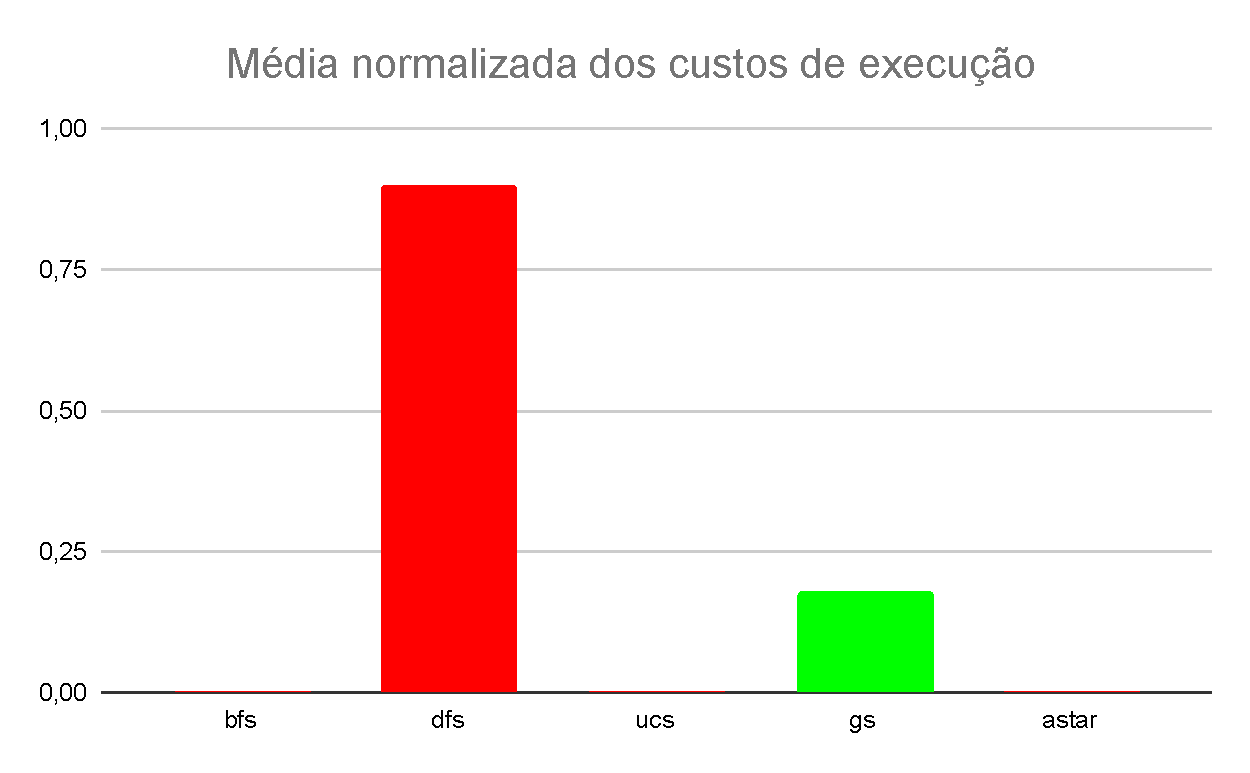
\includegraphics[width=.8\textwidth]{fig/custo.pdf}
  \caption{Média dos custos de execução de todos possíveis \textit{\$scenarios} para cada \textit{\$alg}.}
  \label{fig:custo}
\end{figure}

\begin{figure}[hbt!]
  \centering
  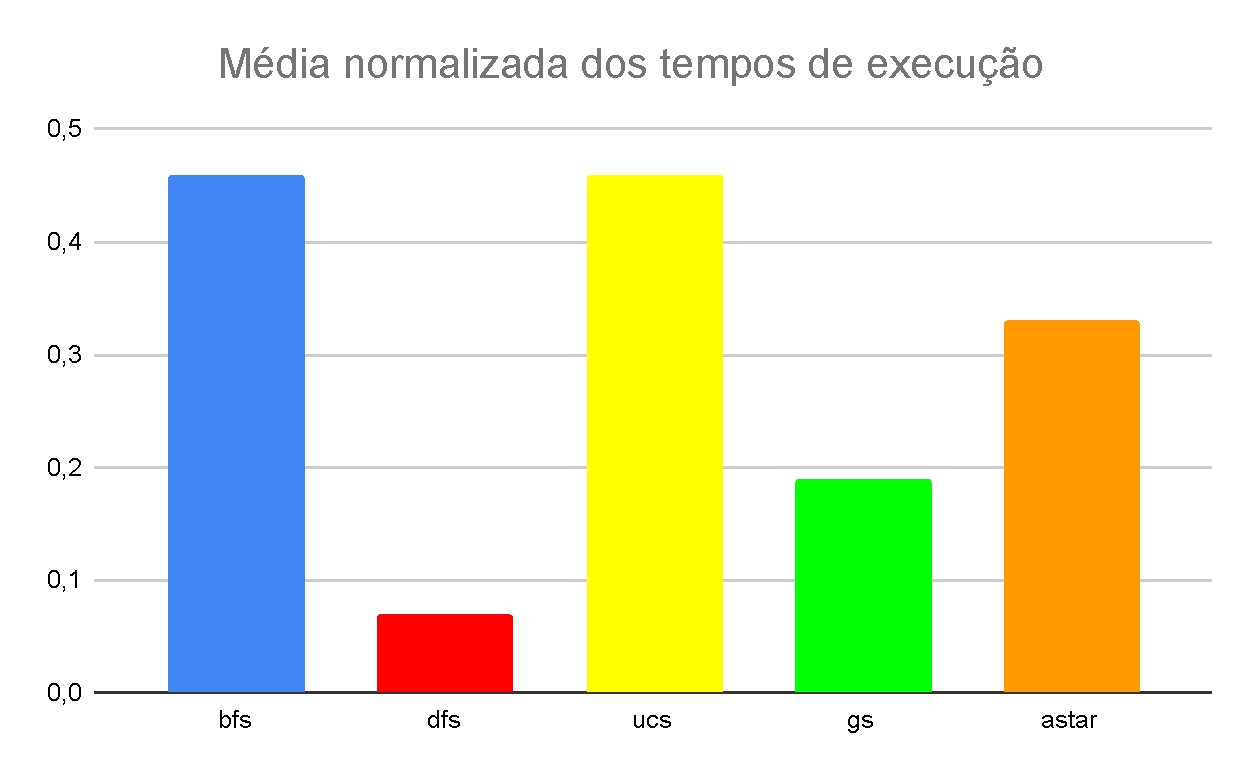
\includegraphics[width=.8\textwidth]{fig/tempo.pdf}
  \caption{Média dos tempos de execução de todos possíveis \textit{\$scenarios} para cada \textit{\$alg}.}
  \label{fig:tempo}
\end{figure}

\begin{figure}[hbt!]
  \centering
  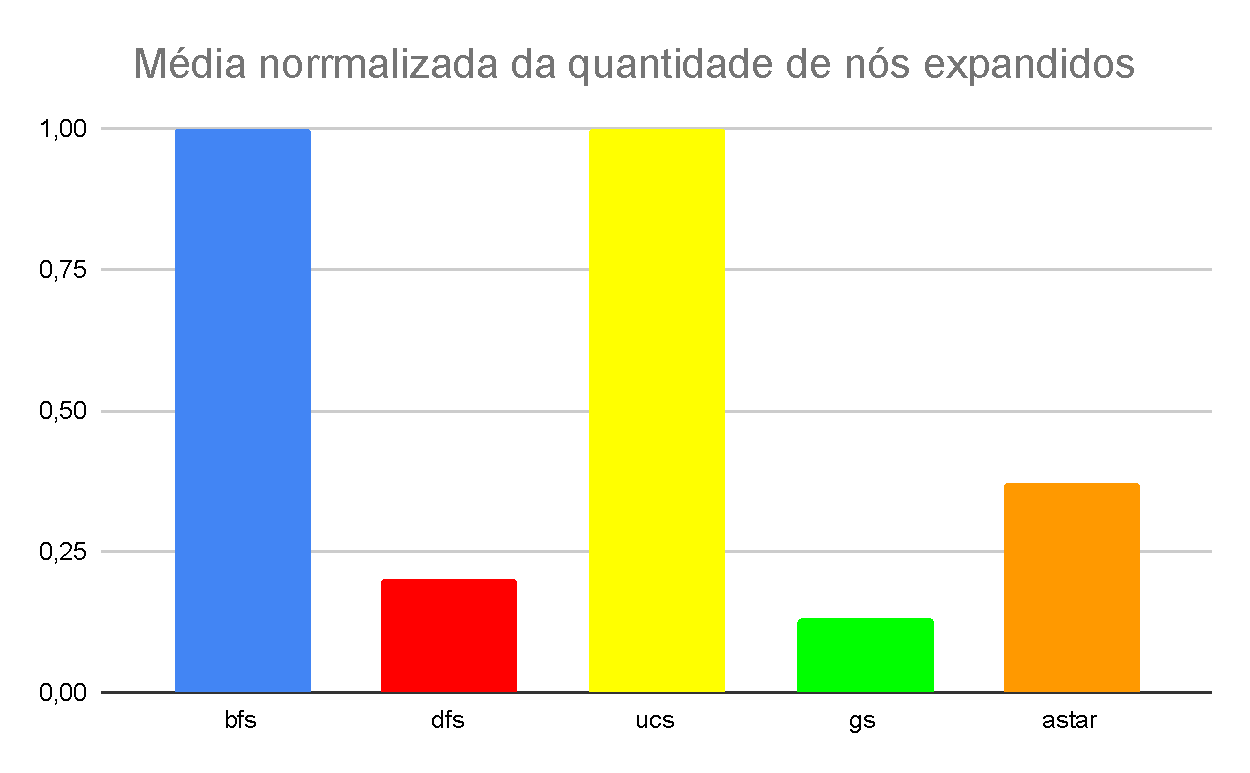
\includegraphics[width=.8\textwidth]{fig/expansao.pdf}
  \caption{Média da quantidade de nós expandidos em todos os possíveis \textit{\$scenarios} para cada \textit{\$alg}.}
  \label{fig:expansao}
\end{figure}


\section{First Page} \label{sec:firstpage}

The first page must display the paper title, the name and address of the
authors, the abstract in English and ``resumo'' in Portuguese (``resumos'' are
required only for papers written in Portuguese). The title must be centered
over the whole page, in 16 point boldface font and with 12 points of space
before itself. Author names must be centered in 12 point font, bold, all of
them disposed in the same line, separated by commas and with 12 points of
space after the title. Addresses must be centered in 12 point font, also with
12 points of space after the authors' names. E-mail addresses should be
written using font Courier New, 10 point nominal size, with 6 points of space
before and 6 points of space after.

The abstract and ``resumo'' (if is the case) must be in 12 point Times font,
indented 0.8cm on both sides. The word \textbf{Abstract} and \textbf{Resumo},
should be written in boldface and must precede the text.

\section{CD-ROMs and Printed Proceedings}

In some conferences, the papers are published on CD-ROM while only the
abstract is published in the printed Proceedings. In this case, authors are
invited to prepare two final versions of the paper. One, complete, to be
published on the CD and the other, containing only the first page, with
abstract and ``resumo'' (for papers in Portuguese).

\section{Sections and Paragraphs}

Section titles must be in boldface, 13pt, flush left. There should be an extra
12 pt of space before each title. Section numbering is optional. The first
paragraph of each section should not be indented, while the first lines of
subsequent paragraphs should be indented by 1.27 cm.

\subsection{Subsections}

The subsection titles must be in boldface, 12pt, flush left.

\section{Figures and Captions}\label{sec:figs}


Figure and table captions should be centered if less than one line
(Figure~\ref{fig:exampleFig1}), otherwise justified and indented by 0.8cm on
both margins, as shown in Figure~\ref{fig:exampleFig2}. The caption font must
be Helvetica, 10 point, boldface, with 6 points of space before and after each
caption.

\begin{figure}[ht]
\centering
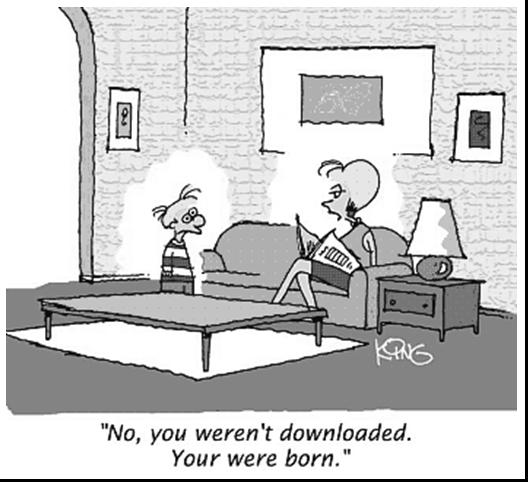
\includegraphics[width=.5\textwidth]{fig1.jpg}
\caption{A typical figure}
\label{fig:exampleFig1}
\end{figure}

\begin{figure}[ht]
\centering
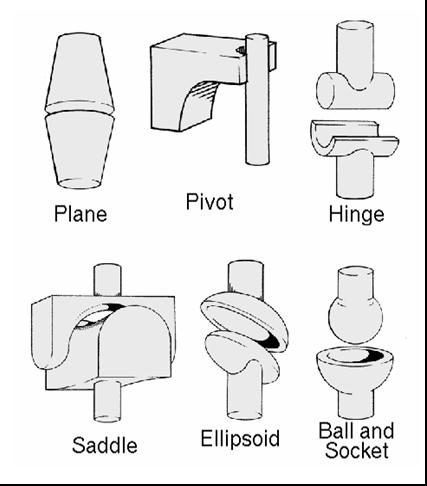
\includegraphics[width=.3\textwidth]{fig2.jpg}
\caption{This figure is an example of a figure caption taking more than one
  line and justified considering margins mentioned in Section~\ref{sec:figs}.}
\label{fig:exampleFig2}
\end{figure}

In tables, try to avoid the use of colored or shaded backgrounds, and avoid
thick, doubled, or unnecessary framing lines. When reporting empirical data,
do not use more decimal digits than warranted by their precision and
reproducibility. Table caption must be placed before the table (see Table 1)
and the font used must also be Helvetica, 10 point, boldface, with 6 points of
space before and after each caption.

\begin{table}[ht]
\centering
\caption{Variables to be considered on the evaluation of interaction
  techniques}
\label{tab:exTable1}
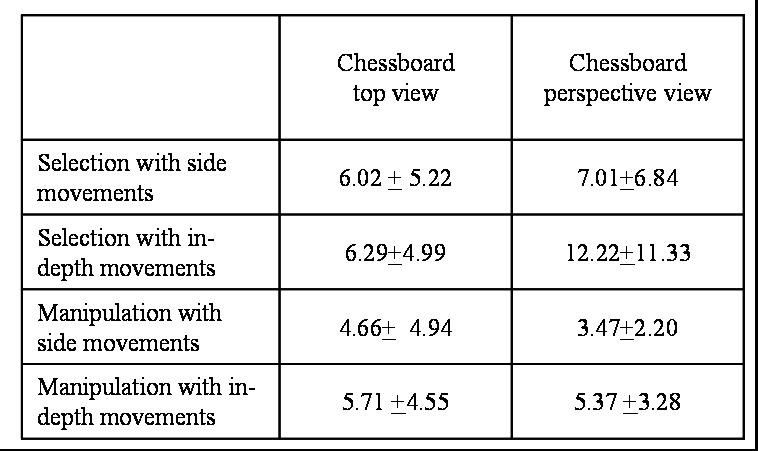
\includegraphics[width=.7\textwidth]{table.jpg}
\end{table}

\section{Images}

All images and illustrations should be in black-and-white, or gray tones,
excepting for the papers that will be electronically available (on CD-ROMs,
internet, etc.). The image resolution on paper should be about 600 dpi for
black-and-white images, and 150-300 dpi for grayscale images.  Do not include
images with excessive resolution, as they may take hours to print, without any
visible difference in the result. 

\section{References}

Bibliographic references must be unambiguous and uniform.  We recommend giving
the author names references in brackets, e.g. \cite{knuth:84},
\cite{boulic:91}, and \cite{smith:99}.

The references must be listed using 12 point font size, with 6 points of space
before each reference. The first line of each reference should not be
indented, while the subsequent should be indented by 0.5 cm.

\bibliographystyle{sbc}
\bibliography{sbc-template}

\end{document}
